\documentclass[a4paper, 12pt]{article}
\usepackage[a4paper,top=1.5cm, bottom=1.5cm, left=1cm, right=1cm]{geometry}
\usepackage[utf8]{inputenc}
\usepackage{mathtext}
\usepackage{amsmath}
\usepackage{amsfonts}
\usepackage[english, russian]{babel}
\usepackage{indentfirst}
\usepackage{longtable}
\usepackage{graphicx}
\graphicspath{{pictures/}}
\DeclareGraphicsExtensions{.pdf,.png,.jpg}
\usepackage{natbib}
\usepackage{mathrsfs}
%\usepackage[europeanresistors, americaninductors]{circuitikz}

\title{Лабораторная работа 1.1.6 Изучение электронного осциллографа}
\author{Михаил Колтаков}
\date{19 октября 2020 г.}

\begin{document}
	\maketitle
	\section*{Цель работы}
		Ознакомление с устройством и работой осциллографа и изучение его основных характеристик
	\section*{Оборудование}
		Осциллограф, генераторы электрических сигналов, соединительные кабели
	\section*{Теория к работе}
		Осциллограф - регистрирующий прибор, в котором исследуемое напряжение преобразуется в видимый на экране график изменения напряжения во времени. С его помощью можно исследовать изменение во времени любых величин, которые могут быть преобразованы в электрические сигналы.
		\par
		Главной частью осциллографа является электронно-лучевая трубка
		\begin{figure}[h]
			\center{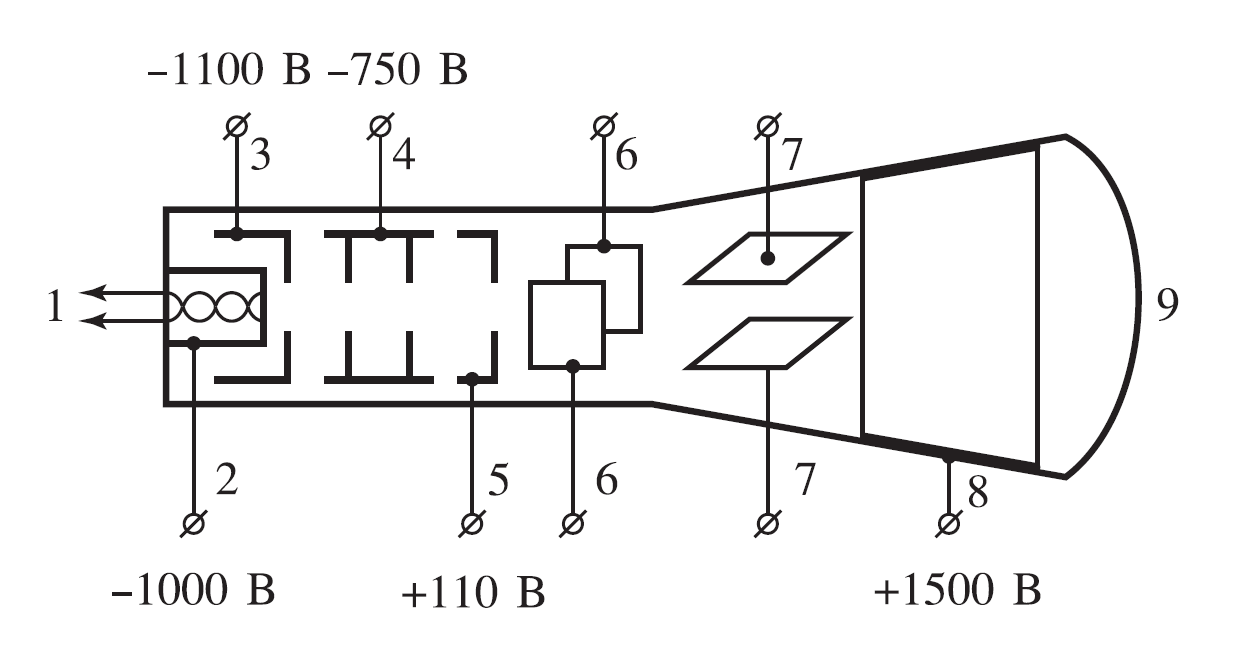
\includegraphics[scale=0.45]{picture1}}
		\end{figure}
	
		Трубка представляет собой откачанную до высокого вакуума колбу, в которой расположены: подогреватель катода 1, катод 2, модулятор 3(электрод, управляющий яркостью изображения), первый (фокусирующий) анод 4, второй (ускоряющий) анод 5, горизонтально и вертикально отклоняющие пластины 6 и 7, третий (ускоряющий) анод 8 и экран 9.
		
		Электронный пучок формируется системой электродов, называемой "электронной пушкой": катод с нагревателем, модулятор, фокусирующий и ускоряющий аноды. Форма, размеры и расположение электродов подобраны таким образом, чтобы разгонять электроны и фокусировать пучок на экране. Экраном осциллографа является покрытая флюоресцирующим веществом стенка трубки, на которую падает электронный пучок. Между пластинами в отклоняющей паре создаётся поле, которое изменяет траекторию полёта электрона в нужном направлении.
		
		Из-за того, что пластины имеют длину и поле между ними имеет конечную величину, осциллограф может корректно "рисовать" только сигналы ограниченной частоты, в нашем случае эта частота примерно равна $10^8\: Гц$.
		
		На практике, однако, максимальная частота ограничена характеристиками усилителя сигнала внутри осциллографа, например, диапазоном значений, в которых коэффициент усиления примерно постоянен(вне этого диапазона коэффициент резко падает). Для учебного осциллографа диапазон частот, в котором он корректно работает  примерно $1-10^6$ Гц
		Осциллограф также имеет две характеристики: АЧХ(амплитудно-частотная характеристика)	и ФЧХ(фазо-частотная характеристика). Для их определения нудно ввести величину $\Delta \Phi_y (f)$ - разность между фазой входного сигнала $U_0$ и фазой колебаний перемещения луча y. Если на вход осциллографа подаётся синусоидальное напряжение амплитудой $U_0$ и частотой $f$, то для перемещения луча на экране можно записать уравнение $y =y_0(f)sin(2 \pi f t + \Delta \Phi_y(f))$, где $y_0(f)$ - амплитуда перемещения луча на частоте $f$. Зная всё это, для канала вертикального отклонения АЧХ можно выразить как $K_y(f) = \frac{y_0(f)}{U_0}$, а ФЧХ как $\Delta \Phi_y (f)$.
		
		Как правило, АЧХ остаётся постоянной в диапазоне частот от $f_{min}$ до $f_{max}$, которые определяют из условий 
		$$\frac{K_y(f_{min})}{K_{y,max}} = \frac{K_y(f_{max})}{K_{y,max}} = \frac{1}{\sqrt{2}}$$
		Непостоянство АЧХ и ФЧХ во всём диапазоне приводят, например, к искажению формы импульсного сигнала высокой частоты при его преобразовании в канале вертикального отклонения осциллографа.
		
		При сложении двух взаимно перпендикулярных колебаний с равными или кратными частотами, поданных на входы осциллографа, луч описывает неподвижные замкнутые кривые, которы называются фигурами Лиссажу. При небольшом нарушении кратности частот фигура начинает двигаться, а при большом картинка становится размытой. Отношение частот на входах равно отношению числа точек касания фигурой горизонтальной прямой к числу точек касания вертикальной прямой.
	\section*{Ход работы}
		1. Подготовим осциллограф к работе.
		
		2. Получим на экране стабильную картину синусоидального сигнала, подаваемого со звукового генератора \\
			a) Подключим звуковой генератор ко входу CH2(Y) и установим на частоту $f \approx 1\: кГц$ \\
			б) Отрегулируем масштаб по вертикали так, чтобы синусоида занимала большую часть экрана. Если это необходимо для установления стационарной картины, переключим режим синхронизации. \\
			в) Измерим длину периода в делениях по шкале X и соотнесём их с положением ручки TIME/DIV, тем самым найдём период колебаний на экране осциллографа. Оценим погрешность измерения частоты таким образом $\delta f$ и сравним полученное значение со значением на экране ЗГ. \\
			г)Проделаем это же ещё несколько раз и результаты занесём в таблицу. \\
			\begin{longtable}[H]{|c|c|c|c|c|c|c|}
				\hline
				$f_{зг},$ Гц & T, дел & TIME/DIV, $дел^{-1}$ & T, с & f, Гц & $\delta f$, Гц & $f - f_{зг}$, Гц \\
				\hline
				1000 & 10,0 & 0,1 мс & $10^{-3}$ & 1000 & 22 & 0 \\
				2000 & 10,2 & 0,05 мс & $0,51 \cdot 10^{-3}$ & 1960 & 41 & -40 \\
				4999 & 10,0 & 0,02 мс & $0,2 \cdot 10^{-3}$ & 5000 & 89 & 1 \\
				9953 & 10,0 & 0,01 мс & $0,1 \cdot 10^{-3}$ & 10000 & 196 & 47 \\
				20096 & 9,8 & 5 мкс & $49 \cdot 10^{-6}$ & 20408 & 350 & 312 \\
				\hline
			\end{longtable}
		3. Найдём отношение максимальной амплитуды, которую может выдавать наш генератор к минимальной. Измерения будем проводить на частоте $f = 1 кГц$ \\
			a) Измерим минимальное и максимальное напряжения: $U_{min} = 30 мВ$, $U_{max} = 55 В$, относительная погрешность при этом $\frac{\delta U}{U} \approx 0,01$. \\
			б) По формуле $\beta_{21} = 20 lg (\frac{U_{max}}{U_{min}})$ найдём отношение предельных напряжений в децибеллах. $\beta \approx 65 дБ$.
		4.Измерим АЧХ осциллографа при разных частотах входного сигнала.\\
			а) На частоте входного сигнала в 1 кГц настроем осциллограф так, чтобы размах синусоиды был равен 4 делениям. \\
			б) Изменяя частоту звукового генератора во всё доступном диапазоне будет фиксировать K(f) при открытом и закрытом режимах входа. Результаты занесём в таблицу. \\
			в) Построим графики $K_{AC}(f)$ и $K_{DC}(f)$ Как видно, пр малых частотах они различаются, а в остальном - совпадают.
			\begin{longtable}[H]{|c|c|c|c|c|c|c|c|c|c|c|c|c|c|}
				\hline
				f, Гц & $5 \cdot 10^{-2}$ & $10^{-1}$ & $0,5$ & 1 & 5 & 7 & 10 & $10^2$ & $10^3$ & $10^6$ & $1,6 \cdot 10^7$ & $2 \cdot 10^7$ & $2,6 \cdot 10^7$ \\
				\hline
				lg f & -1,3 & -1,0 & -0,3 & 0,0 & 0,7 & 0,8 & 1,0 & 2,0 & 3,0 & 6,0 & 7,2 & 7,3 & 7,4 \\
				$2 U_{AC}$, дел & 0,00 & 0,08 & 0,20 & 1,20 & 2,40 & 3,40 & 4,00 & 4,00 & 4,00 & 4,00 & 3,62 & 2,30 & 0,036 \\
				$K_{AC} = \frac{U_{AC}}{U_0}$ & 0,00 & 0,02 & 0.05 & 0,3 & 0,6 & 0,85 & 1,0 & 1,0 & 1,0 & 1,0 & 0,91 & 0,58 & 0,144 \\
				$2U_{DC}$, дел & 4,00 & 4,00 & 4,00 & 4,00 & 4,00 & 4,00 & 4,00 & 4,00 & 4,00 & 4,00 & 3,62 & 2,30 & 0,36 \\
				$K_{DC}= \frac{U_{DC}}{U_0}$ & 1,00 & 1,00 & 1,00 & 1,00 & 1,00 & 1,00 & 1,00 & 1,00 & 1,00 & 1,00 & 0,91 & 0,58 & 0,144 \\
				\hline
			\end{longtable}
			\begin{figure}[h]
				\center{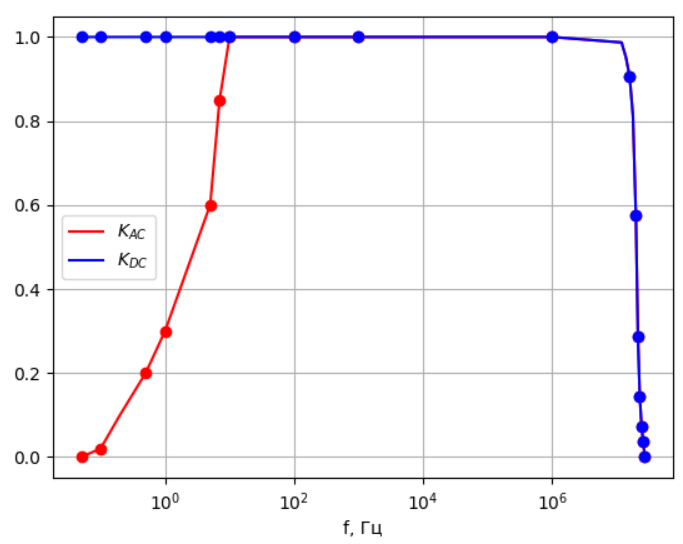
\includegraphics{picture2}}
			\end{figure}
		5. Изучим влияние АЧХ на искажение сигнала.
			а) Установим звуковой генератор в режим меандров и на частоту 1 кГц. \\
			б) Будем менять частоту во всём диапазоне частот и зарисуем получившиеся на экране осциллографа картинки. 
			\begin{figure}[h]
				\center{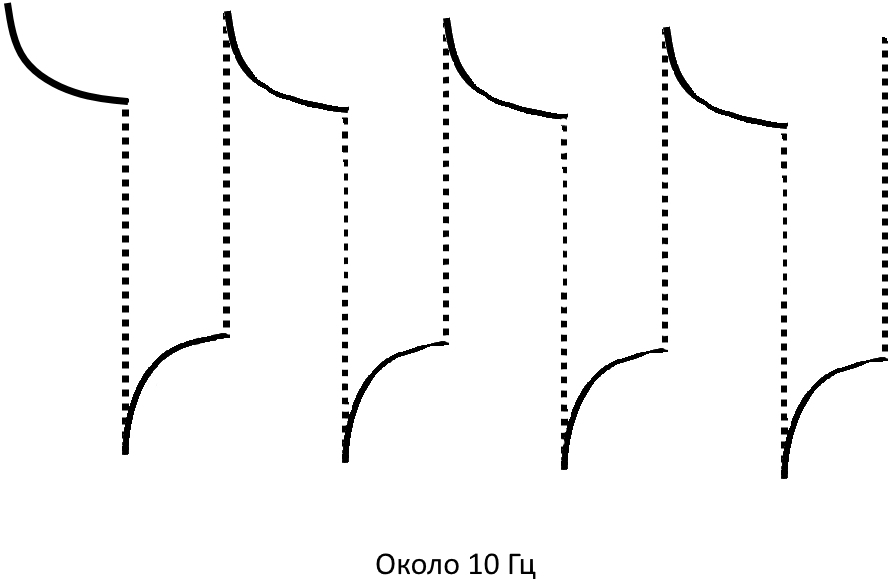
\includegraphics[scale=0.45]{graph2}}
			\end{figure}
			\begin{figure}[h]
				\center{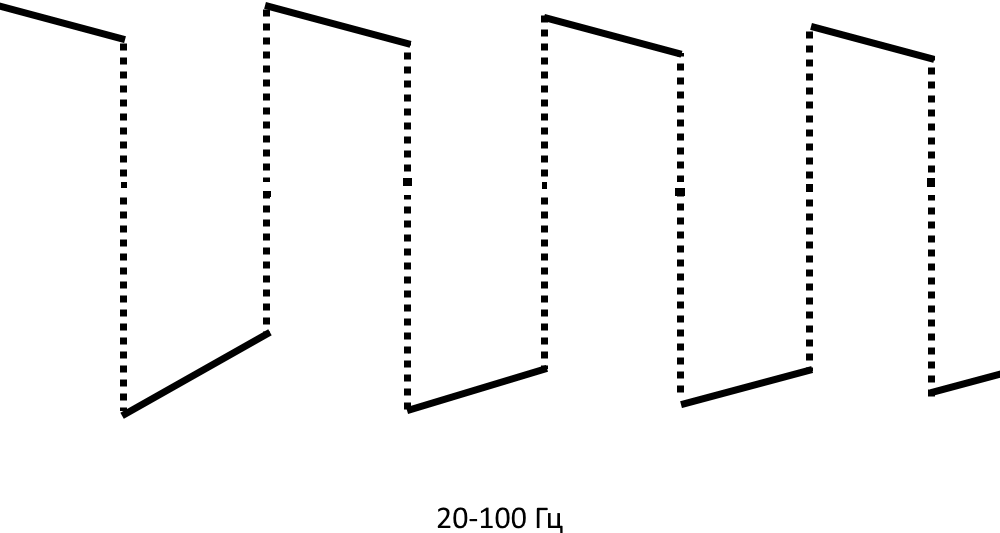
\includegraphics[scale=0.45]{graph1}}
			\end{figure}
			\begin{figure}[h]
				\center{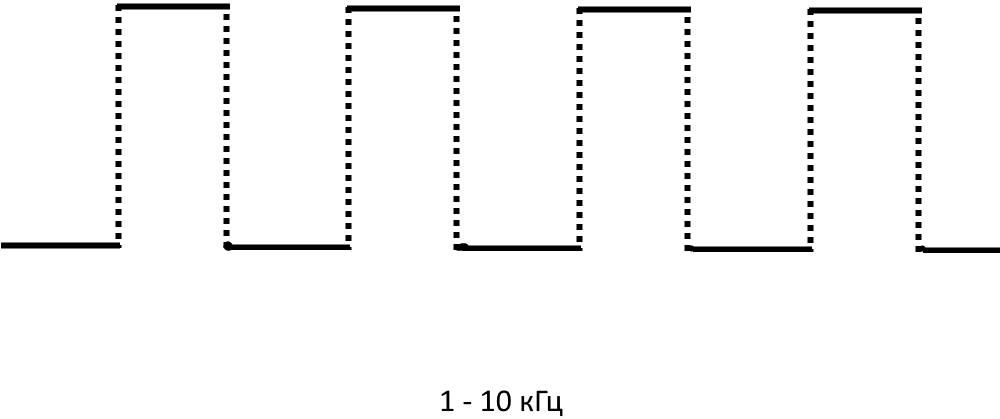
\includegraphics[scale=0.45]{graph3}}
			\end{figure}
			\begin{figure}[h]
				\center{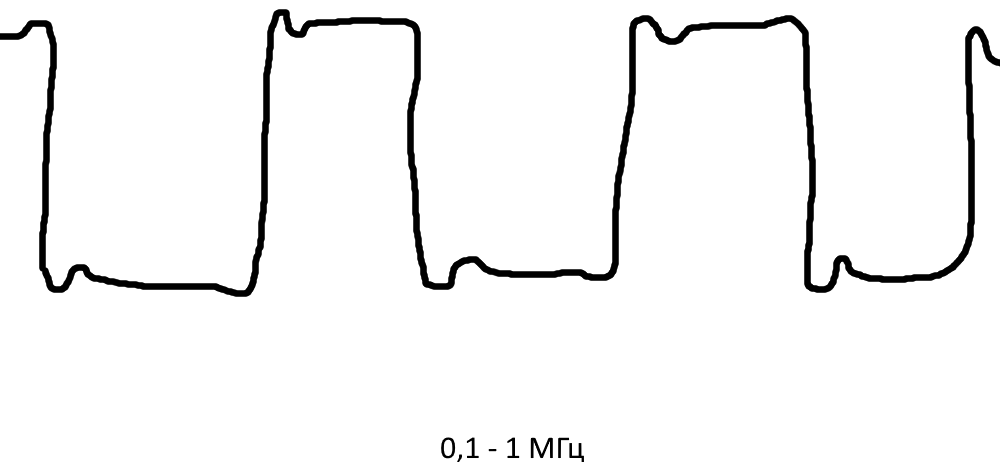
\includegraphics[scale=0.45]{graph4}}
			\end{figure}
			\\
			\\
			\\
			\\
			\\
			\\
			\\
			\\
			\\
			\\
			\\
			\\
			\\
			\\
			\\
			\\
			\\
			\\
			\\
			\\
			\\
			\\
			\\
			\\
			\\
			\\
			\\
			\\
			в) Так как меандр создаётся комбинацией большого числа синусоид разных амплитуд, синхронизированных не менее, чем до десятой гармоники, которые можно разложить в ряд Фурье таким образом:
			$$y(x)= c_1 \sum_{k = 1}^{\infty} \frac{sin(2 \pi (2k - 1)ft)}{2k - 1}$$
			Как видно, коэффициенты при гармониках более высоких частот меньше, чем при более низких, поэтому гармоники низких частот задают общую форму волны( "начала" и "концы" каждого "прямоугольника"), а гармоники высоких частот "выравнивают" горизонтальные участки прямой и т. к. АЧХ у осциллографа меняется в зависимости от частоты входящего сигнала, то на высоких частотах гармоники с высокими частотами обращаются в 0 и волна начинает больше напоминать гармонику. Особенно хорошо это заметно в начале каждого "прямоугольника", т. к. тогда все гармоники имеют одинаковую фазу. А на низких частотах гармоники низких частот начинают влиять меньше, т. к для них АЧХ падает и поэтому концы "прямоугольников" начинают быть не на той же высоте, что и их начала.
			
		6. Измерим ФЧХ осциллографа \\
			а) Подадим с помощью разветвителя одну и ту же синусоиду на оба входа осциллографа. С помощью ручек VOLTS/DIV добьёмся того, чтобы на экране была видна линия, наклонённая к горизонтали на угол 45 градусов. \\
			б) Изменяя частоту во всём доступном диапазоне генератора, найдём те места, где прямая будет превращаться в эллипс. Измерим отношение длины отрезка, соединяющего точки пересечения эллипса с осью ординат к амплитуде эллипса(разности ординат самой высокой и самой низкой его точек). Занесём результаты в таблицу \\
			\\
			\\
			\\
			\begin{longtable}{|c|c|c|c|c|c|c|c|}
				\hline
				f, Гц & 10 & $10^2$ & $10^3$ & $10^4$ & $10^5$ & $5 \cdot 10^5$ & $10^6$ \\
				\hline
				lg f & 1,0 & 2 & 3,0 & 4,0 & 5,0 & 5,7 & 6,0 \\
				$|2y_0|$, дел  & 0 & 0 & 0 & 0 & 0,3 & 1,0 & 2,1 \\
				$|2A_y|$, дел & 4,0 & 4,0 & 4,0 & 4,0 & 4,0 & 4,0 & 4,0 \\
				$arcsin|\frac{y_0}{A_y}|$, градусы & 0 & 0 & 0 & 0 & 4,47 & 14,48 & 31,67 \\
				$|\Delta \phi|$, градусы & 0 & 0 & 0 & 0 & 4,47 & 14,48 & 31,67 \\
				\hline
			\end{longtable}
			в) Построим график $\Delta \phi(lg f)$ в логарифмическом масштабе.
			\begin{figure}[h]
				\center{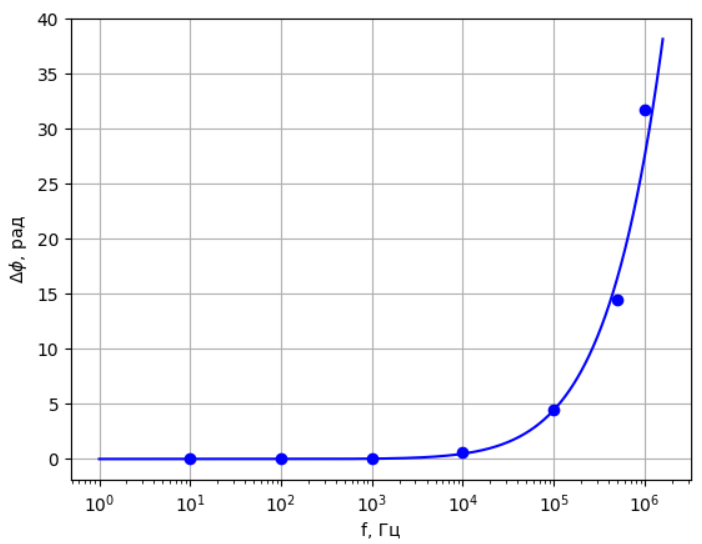
\includegraphics{picture3}}
			\end{figure}
		
		7. Пронаблюдаем фигуры Лиссажу, подавая на сходы осциллографа синусоиды с разными частотами. \\
			а) Пронаблюдаем кривые при отношениях поданных частот 1:1, 2:1, 3:1 и 3:2. В них наблюдаются предполагаемые количества(как отношение частот сигналов) точек касания воображаемых вертикальной и горизонтальной прямых.
			Вот так выглядят эти фигуры(картинка после вывода)
			\begin{figure}[h]
				\center{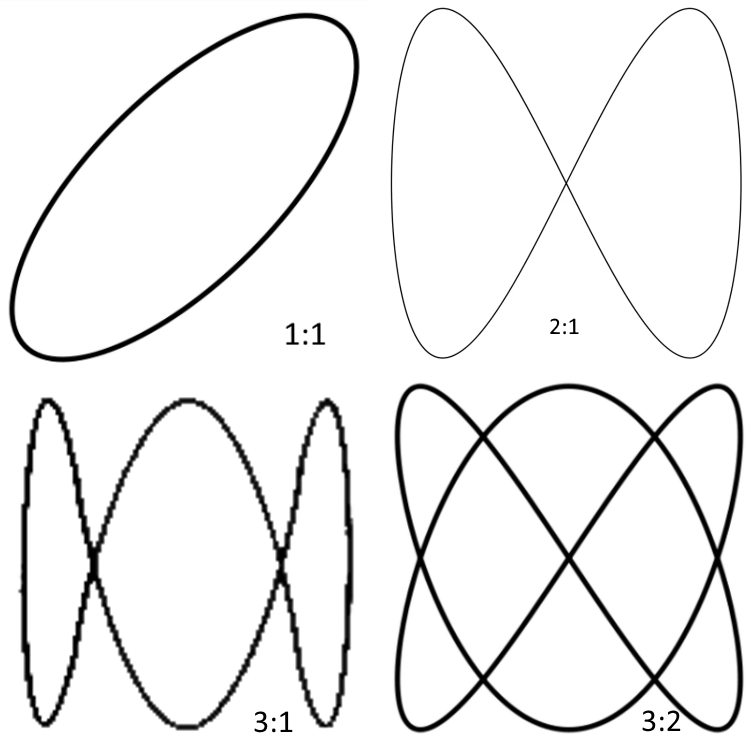
\includegraphics{figures}}
			\end{figure}
	\section*{Вывод}
		Мы ознакомились с устройством и принципами работы осциллографа, изучили, как он ведёт себя в разных критических случаях и исследовали фигуры Лиссажу с помощью него.
\end{document}
